\documentclass[conference]{IEEEtran}

% correct bad hyphenation here
\hyphenation{op-tical net-works semi-conduc-tor}
  
\usepackage[utf8]{inputenc} 
\usepackage[pdftex]{graphicx}
\usepackage[version=3]{mhchem}
\usepackage{caption}
\usepackage{chemfig}
\usepackage{enumerate}
\usepackage{multirow}

\DeclareCaptionLabelFormat{lc}{\MakeLowercase{#1}~#2}
\captionsetup{labelfont=sc,labelformat=lc}

%Algoritmo
\usepackage[ruled,lined,linesnumbered]{algorithm2e}
\SetKwInOut{Input}{Input}
\SetKwInOut{Output}{Output}


\begin{document}
	
\title{Multi objective evolutionary algorithms applied to protein structure prediction problem}

\author{
	\IEEEauthorblockN{Vidal D. da Fontoura, Ricardo H. R. de Lima, Aurora T. R. Pozo, Roberto Santana}
	
	\IEEEauthorblockA{
		Computer Science Department\\
		Federal University of Paraná - UFPR\\
		Curitiba - PR, Brazil}
	
	%TODO arrumar email Roberto
	\IEEEauthorblockA{Email: \{vdfontoura, rhrlima, aurora\}@inf.ufpr.br, roberto.santana@ehu.es}
	}



% make the title area
\maketitle

\begin{abstract}

Many heuristics methods have been successfully applied to the PSP using simplified models for representation of the problem. This methods usually minimize the free energy of a protein structure. This study aimed the application of multi objective genetic algorithms combined with a relative representation for the 2D-HP prediction model. Experiments were conducted with two well-known algorithms: Non-dominated sorting Genetic Algorithm II (NSGAII) and Indicator-Based Evolutionary Algorithm (IBEA). Moreover, the algorithms are evaluated and compared using different genetic operators.

\end{abstract}

% no keywords

\IEEEpeerreviewmaketitle


\section{Introduction}

The proteins have a fundamental task in the nature. These structures, made of amino-acids, participate in many of the most important tasks of the living cells. Proteins guarantee the correct functioning of a large number of biological entities in nature. The protein structure is the result of the so-called protein folding process in which the initially unfolded chain of amino-acids is transformed into its final structure. Under suitable conditions, this structure is uniquely determined by its sequence \cite{}.%TODO COLOCAR REFERNCIA ROBERTO.


A protein, is a macromolecule built by a chain of amino acids. The biological function of a protein is determined by the way it is folded into a specific structure. Understanding how proteins fold is of great importance to Biology, Biochemistry and Medicine. Considering the full analytic atomic model of a protein, it is still not possible to determine the exact structure of real-world proteins, even with the most powerful computational resources \cite{lopes2008evolutionary}.


In this scenario, different heuristic approaches have been developed to decrease the computational complexity related to the protein structure determination process. Between this approaches, there are studies that explore the protein structure prediction combined with evolutionary algorithms like for example, the author of \cite{li2012genetic} proposed an mono objective EA (Evolutionary Algorithm) working with a local search strategy for the PSP Problem using the simplified model Hydrophobic-Polar (HP). Then \cite{soares2011investigating} proposed an multi objective algorithm in tables and compares its performance with the NSGAII \cite{deb2002fast}, optimizing two energy functions, both very important for the the folding process: the van der Walls and Electrostatic functions. The author of \cite{gabriel2012algoritmos} also proposes the using of a multi objective algorithm in tables, similar to the proposed method by \cite{soares2011investigating}, however, using the HP model for the representation and solution evaluation.


This work proposes the application and comparison of the multi objective evolutionary algorithms NSGAII and IBEA \cite{zitzler2004indicator} aiming as a first objective minimizing the energy calculated from the HP model, and as second objective minimizing the euclidean distance between amino acids of a protein.


This work is organized as follows. Section \ref{sec:psp_problem} presents the PSP problem, the HP model and its relative representation. Section \ref{sec:evol_algs} talks about genetic algorithms and multi objective optimization. Section \ref{sec:compared_methods} shows the compared methods. Section \ref{sec:experiments} presents the conducted experiments. Section \ref{sec:related_works} talk about some related works. Finally, Section \ref{sec:conclusion} concludes the analysis about the experiments and mention the possible improvements to this study.


\section{Protein Structure Prediction Problem}
\label{sec:psp_problem}


The Protein Structure Prediction (PSP) is about the determination of the final structure of a protein when only a sequence of amino acid residues is given \cite{dorn2014three}. A computational approach to predict the structure of a protein demands a model that represents it abstractly, in a given level of details. Based on well-established thermodynamical laws, the prediction of the structure of a protein is modeled as the minimization of the corresponding free-energy with respect to the possible conformations that a protein is able to attain. Formally, the native conformation of a protein is defined as that in which the free-energy is minimal. The amount of details of the structure depends on the choices done about the model. For instance, a protein could have a spatial representation of all its atoms, all its atoms but hydrogen, only the backbone without side-chain, or a simple hydrophobic-polar elements embedded in a lattice \cite{lopes2008evolutionary}.


\subsection{Hydrophobic-Polar Model}

The Hydrophobic-Polar model, or HP model, was developed by Lau and Dill \cite{lau1989lattice}. Its a network model, among others, which is used in researches for the PSP, and, like others, is a model of protein representation that has simplifications. The model considers two types of residues: hydrophobic (H) and Hydrophilic or Polar (P). A protein is considered a sequence of these two types of residues, which are located in regular lattice models forming self-avoided paths. In this model, the main concept is the neighborhood concept. Given a pair of residues, they are considered neighbors if they are adjacent  either in the chain (connected neighbors) or  in the lattice but not connected in the chain (topological neighbors) \cite{santana2008protein}. The Figure \ref{fig1} shows an example of a sequence in the HP model, where the black dots represents the H residues, and the white dots the P residues. Connected neighbors are represented by the continuous line, while the topological neighbors are highlighted by dashed ellipses.

\begin{figure}[ht]
	\centering
	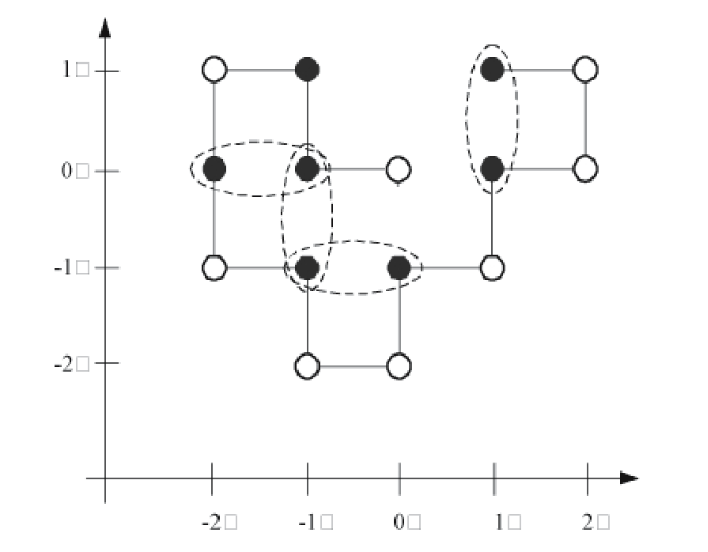
\includegraphics[width=2.5in]{figures/figure1.png}
	\caption{Hypothetical conformation of a chain of 15 amino acids using the 2D-HP model \cite{lopes2008evolutionary}}.
	\label{fig1}
\end{figure}

In the HP model, for each pair of residues, some values are given for the energy depending of the pair: $\epsilon_{HH}=1$ and $\epsilon_{PP} = \epsilon_{HP} = 0$. The free-energy of a conformation is inversely proportional to the number topological neighbors. Consequently, minimizing the free-energy is equivalent to maximize the number of topological neighbors \cite{lopes2008evolutionary}.


\subsection{Relative Representation}


The relative representation for the HP model is based on the construction of the protein structure using a sequence of directions. In this approach, each residue has its position placed relative to the previous one \cite{lopes2008evolutionary}. For a chain of $N$ residues, starting from the first witch has a fixed position, every subsequent residue is placed according to a given direction. For the 2D-HP model only three directions are possible: 


\begin{itemize}
	\item Forward: to continue walking on the same direction;
	\item Turn Right: place the residue at right of the previous;
	\item Turn Left: place the residue at the left of the previous;
\end{itemize}


For each residue that is placed, the actual direction is updated. This way, the commands "Forward", "Turn Right" and "Turn Left" will all be based on the previous residue, as the Figure \ref{fig2} shows.

%TODO mudar figura para ingles
\begin{figure}[ht]
	\centering
	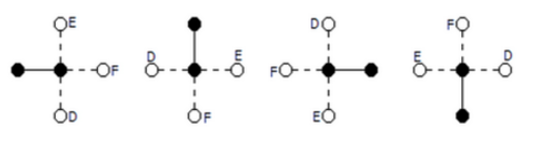
\includegraphics[width=2.5in]{figures/figure2.png}
	\caption{Example of relative representation, where F means the movement Forward, R means Right and L means Left.}
	\label{fig2}
\end{figure}


\section{Multi objective Evolutionary Algorithms}
\label{sec:evol_algs}


Evolutionary Algorithm (EA) is a optimization and search technique, highly parallel, inspired by the Darwinian principle of natural selection and genetic reproduction. The nature principles that inspire the EAs are simple. According to the theory of C, Darwin, the principle of natural selection favors individuals with high fitness, therefore, with high probability of reproduction. Individuals with more descendants have more chance to perpetuate their genetic code in future generations. The genetic codes is what gives the identity of each individual and are represented in the chromosomes. These principles are used in the construction of computational algorithms, that searches for better solutions given a specific problem by the evolution of a population of solutions coded in artificial chromosomes -- data structures used to represent a feasible solution for a given problem in the algorithm execution \cite{pacheco1999algoritmos}.


Real world problems commonly have multiple objectives to minimized/maximized and are present in most knowledge areas. To optimize multi objective problems, are considered two or more objectives witch usually are conflicting. To these problems is impossible to find one unique solution. A set of solutions is reached evaluating the Pareto dominance relation \cite{pareto} between the solutions. The main objective is to find the solutions that are non-dominated by any other. A solution dominates other, if and only if, it was better in at least one of the objectives, without being worst in any of the objectives. The set of non-dominated solutions constitutes the Pareto Front. Finding the the real Pareto Front is a NP-hard problem \cite{fonseca2005tutorial}, this way, the objective is to find a good approximation of this front.


Multi-Objective Evolutionary Algorithms (MOEAS) are extensions of EAs to multi objective problems that applies the concepts of Pareto dominance to create different strategies to evolve and diversify the solutions. In this work were used two MOEAs: NSGAII \cite{deb2002fast} and IBEA \cite{zitzler2004indicator}.


\subsection{Non-dominated sorting Genetic Algorithm II}


The main characteristic of this algorithm is a strong elitism mechanism, classifying at each generation every solution in different fronts according with the non-dominance relation (line 15 of Algorithm \ref{alg:nsgaII}). After the classification, solutions from the first front, are non-dominated by any other solution. Solutions from the second front are dominated only by the solutions of the first front, and so on. For solutions of the same front, the algorithm uses a Crowding Distance operator to calculate how distant are the neighbors of a given solution (line 19 of Algorithm \ref{alg:nsgaII}). Solutions with high values of Crowding Distance have priority, because they will contribute more to the population's diversity. The binary tournament selects solutions from the small front with the higher values of Crowding Distance. A new population is generated using the crossover and mutation operators (line 25 of Algorithm \ref{alg:nsgaII}).


\begin{algorithm}[ht]
	\Input{N: Population Size \\T // Max evaluations}
	
	\Output{P: Set of non-dominated solutions}
	
	\Begin{
		$P_0 \gets CreatePopulation(N);$\\
		$CalculateFitness(P_0);$\\
		$FastNonDominatedSort(P_0);$\\
		$Q_0 \gets 0;$\\
		\While{$Q_0 < N$}{
			$Parents \gets BinaryTournament(P_0);$\\
			$Children \gets CrossoverMutation(Parents);$\\
			$Q_0 \gets Children;$\\
		}
		$CalculateFitness(Q_0);$\\
		
		$t \gets 0;$\\
		\While{$t < T$} {	
			$R_t \gets P_t \cup Q_t;$\\
			$Fronts \gets FastNonDominatedSort(R_t);$\\
			$P_{t+1} \gets 0;$\\
			$i \gets 0;$\\
			
			\Enqto{$P_{t+1} + Front_i  < N$} {
				$CrowdingDistanceAssignment(Front_i);$\\
				$P_{t+1} \gets P_{t+1} \cup Front_i;$\\
				$i \gets i + 1;$\\
			}
			$CrowdingDistanceSort(Front_i)$;
			$P_{t+1} \gets P_{t+1} \cup Front_i[1:(N -P_{t+1})]$
			
			$Parents \gets BinaryTournament(P_{t+1})$;\\
			$Q_{t+1} \gets CrossoverMutation(Parents)$;
			
			$t \gets t +1$;
		}
	}
	\caption{NSGAII}
	\label{alg:nsgaII}
\end{algorithm}


\subsection{IBEA (Indicator-Based Evolutionary Algorithm)}


In the multi-objective optimization context, optimizing consists in find a front with a good approximation to the true Pareto front. However, there is no general definition about what is the true Pareto front. This way, indicators have been used to evaluate the quality of a approximation front. The \textit{hypervolume} is a example of indicator to the evaluation and comparison of fronts.


The IBEA is an algorithm that considers the optimization by the use of quality indicators. The indicator is the way used to evaluate the non-dominated set of solutions \cite{figueiredo2013algoritmo}. To use the IBEA it is necessary define which indicator will be used to associate each ordered pair of solutions to a scalar value. One of the most used indicators is the \textit{hypervolume} due to its capacity of evaluate the convergence and diversity at the same time of the search process \cite{ishibuchi2008evolutionary}.


\begin{equation} \label{eq:ibea_fitness}
	F(x_i) = \sum_{x_j \in (P-x_i)} {-e^\frac{-I_{Hy}(x_j,x_i)}{k}}
\end{equation}


For the IBEA fitness calculation (Equation \ref{eq:ibea_fitness}), $k$ is a parameter commonly used with a value of 0.05. The value for $F(x_i)$ corresponds to a quality loss measure of the approximation to the Pareto front if the solution $x_i$ was removed of the population \cite{figueiredo2013algoritmo}, based on the value of the quality indicator $I_{Hy}$, in this case, the \textit{hypervolume}. Based on the fitness calculation described above, the basic IBEA algorithm consists in iteratively do the selection (line 10 of Algorithm \ref{alg:ibea}), crossover, mutation (line 11 of Algorithm \ref{alg:ibea}) and environment selection, removing the worst individual from the population and updating the values of fitness of the remaining individuals (lines 4 to 8 of Algorithm \ref{alg:ibea}).


\begin{algorithm}[h]
	
	\Input{N: Population Size \\T: Max Evaluations\\ k: Scale factor of Fitness}
	
	\Output{P: Set of non-dominated solutions}
	
	$P \gets$ CreatePopulation($N$)\\
	$m \gets 0$\\
	CalculateFitness($P$)\\ 	
	
	\While{Size($P$) $> N$} {
		$x^* \gets$ WorstIndividualByFitness()\\
		RemoveFromPopulation($x^*$, $P$)\\
		CalculateFitness($P$)\\
	}
	
	\If{$m \ge T$ or other stop criterion is reached}{
		\Return $A$\\	
	}
	
	$\overline P \gets$ BinaryTournament($P$)\\
	
	$P \gets$ CrossoverMutation($\overline P$)\\
	$m \gets m+1$

	\caption{IBEA}
	\label{alg:ibea}
\end{algorithm}


\footnotetext[1]{\textit{Hypervolume}: Proposed quality indicators used in the study of \cite{zitzler1998multiobjective}, denoted as the "size of the covered search space". This indicator has two important advantages in relation to others \cite{zitzler2007hypervolume}: 1 - Sensitive to any kind of improvement in the approximation set in relation to other set. 2 - As result of 1, the indicator guarantee that for any approximation set $A$ that has high values of hypervolume, also has all the solutions of the true Pareto front.}


\section{Compared Methods} \label{sec:compared_methods}


The proposed method consists in the application of the algorithms NSGAII and IBEA to the PSP problem using the relative representation applied to the HP model. The multi-objective optimization framework jMetal \cite{jMetal} was used, it presents implementation of the used MOEAs and a easy way to personalize them. To evaluate the generated solutions, a evaluation mechanism was implemented considering two objectives:


\begin{enumerate}[I]
	\item Maximize the number of topological neighbors HH (main objective);
	\item Minimize the maximum euclidean distance between residues (secondary objective).
\end{enumerate}


The first objective guide the search aiming find a solution that generates a structure where the energy value is minimum (maximizing the number of topological neighbors HH), this way, obtaining a structure closer of the native conformation of the protein. The second objective allows to differ solutions with the same value of energy but with different compression degrees. The more compact was the max value of euclidean distance, more compact will be the generated conformation.


The chromosomes are represented by integer vectors where the genes specify which direction, related to the previous residue, the next one should be placed. The genes can assume one of three values 0, 1 and 2, where 0 means the next residue should be placed at right of the previous one, 1 means the next residue should be placed in front of the previous and 2 means the next residue should be placed at left of the previous one. The Figure \ref{fig_sim} demonstrate a example of a possible chromosome to a chain of 10 residues and its generated conformation.

%TODO mudar para ingles
\begin{figure}[ht]
	\centering
	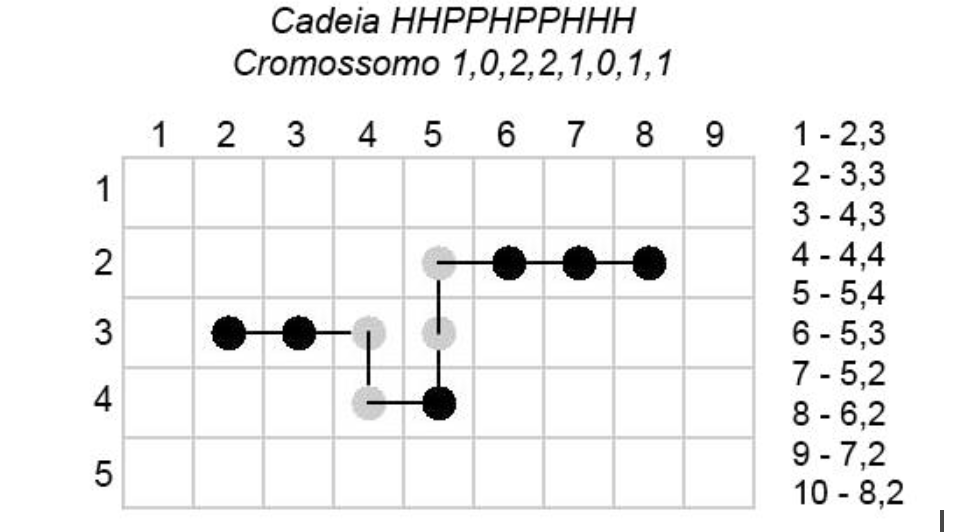
\includegraphics[width=2.5in]{figures/figure3.png}
	\caption{Example of a conformation generated by a chromosome with relative representation.}
	\label{fig_sim}
\end{figure}


The relative representation it is subject to the generation of infeasible solutions using the HP model. A solution is considered infeasible when a residue 'collides' with another already placed on the lattice. A simple mechanism for repairing these situations was developed, the code can be seen in the Algorithm \ref{algo:reparacao}.


\begin{algorithm}[h]
	Obtains the direction the next residue should be placed.\\
	Verifies if this direction will cause collision.\\
	If the a collision is identified, a new direction is used.\\
	Repeat the step 2 and 3, until be possible to place the next residue, or if all directions were tested and cause collisions.\\
	If was possible to place the next residue, the mechanism reached success, if not, the solution is considered infeasible and it will be penalized in the evaluation process.
	\caption{Mechanism to repair infeasible solutions}
	\label{algo:reparacao}
\end{algorithm}


This mechanism was implemented because in early experiments was observed that the number of infeasible solutions was too big. It is necessary mention that the even with the mechanism to repair solutions, there are still infeasible solutions because the mechanism can't always repair. Yet, infeasible solutions are penalized by subtracting the number of collisions to the quantity of topological neighbors.


To evaluate and compare the performance of the multi-objective algorithms, quality indicators are commonly used. In this study was used the hypervolume indicator, which considers the volume of the search space dominated by the true front \cite{zitzler2003performance}. The high the hypervolume is, better the quality of the front found by one of the algorithms.


\section{Experiments and Results} \label{sec:experiments}


Experiments were conducted using the algorithms NSGAII and IBEA presented in Section \ref{sec:compared_methods}. A variation and combination of the parameters was made to find the best configuration of each algorithm. The result was 120 different configurations for the IBEA and 60 fo the NSGAII, since it does not use auxiliary population. The Table \ref{tab:tuning} shows the values that vary in the experiments.

\begin{table}[h]
	\centering
	\caption{Parameters used in the experiments}
	\label{tab:tuning}
	\begin{tabular}{|c|c|}
		\hline
		{\bf Parameter} & {\bf Values}                 \\ \hline
		Population       & 200, 250, 300, 350, 400           \\
		\hline
		Pop Aux. (IBEA)        & 200,300                       \\ \hline
		Evaluations      & 40000, 60000, 70000, 100000      \\ \hline
		Crossover      & SinglePoint, TwoPoints, Uniform \\ \hline
		Cross \%.      & 90\%                          \\ \hline
		Mutation         & BitFlip                       \\ \hline
		Mut \%.       & 0.01\%                        \\ \hline
	\end{tabular}
\end{table}


For comparison, it was used a 64-length chain, the most complex chain used in the studies developed by Liet al. \cite{li2012genetic}. The formula below represents the sequence of amino acids:

\begin{center}
	\begin{small}
		\noindent \ce{H12PHPHP2H2P2H2P2HP2H2P2H2P2HP2H2P2H2P2HPHPH12} 
	\end{small}
\end{center}

Because it is stochastic algorithms, each configuration was executed 30 times to evaluate if the behavior maintain itself in the executions, resulting 30 approximated fronts. For each front, the duplicated and dominated solutions were removed. The resulting fronts were normalized, to harmonize the objective scales. The calculation for the normalization is presented in Equation \ref{eq:calcNorma}.


\begin{equation} \label{eq:calcNorma}
	Xnorm = (X - MIN) / (MAX - MIN)
\end{equation}


Where $X$ is the value of one of the objectives, $MIN$ and $MAX$ are the smallest and biggest values found for the selected objective. The normalization is necessary because the values for the two objectives are in different scales. The normalization make possible to guarantee that the objective values will be at a 0 and 1 scale. This way, calculate the hypervolume avoids the prioritization of disproportional scales.


The values of hypervolume were calculated for each front generated by the 30 executions of each configuration. The average, standard deviation, min and max values were calculated for each configuration. The Table \ref{tab:media} shows the hypervolume value of the best configuration obtained for each algorithm and the result of the statistical Kruskal-Wallis test \cite{kruskal1952use} between them. The Table \ref{tab:bestConfigs} presents the best configuration for each algorithm.


\begin{table}[h]
	\centering
	\caption{Best results obtained}
	\label{tab:media}
	\scalebox{0.9}{
	\begin{tabular}{|c|c|c|c|c|c|}
		\hline
		Algorithm & Average        & Std Dev & Min & Max & \multicolumn{1}{l|}{Kruskal-Wallis} \\ \hline
		NSGAII    & 0.5222       & 0.0429        & 0.4496 & 0.6025 & \multirow{2}{*}{TRUE}        \\ \cline{1-5}
		IBEA      & {\bf 0.5855} & 0.0711        & 0.4739 & 0.7799 &                              \\ \hline
	\end{tabular}}
\end{table}


It is possible to observe in the average values of hypervolume, with statistical difference by the Kruskal-Wallis test, the algorithm IBEA has a bigger coverage of the search space when compared to the NSGAII. This way, can be said the IBEA obtained a better performance over the NSGAII, because the front generated by the IBEA dominates the front generated by the NSGAII.


\begin{table}[h]
	\centering
	\caption{Best parameter configurations for the Algorithms}
	\label{tab:bestConfigs}
	\scalebox{0.9}{
	\begin{tabular}{|c|c|c|p{0.4cm} |p{1.5cm}|p{1.3cm}|}
		\hline
		\textbf{Algorithm} & 	\textbf{Evaluations} & 	\textbf{Population} & 	\textbf{Pop Aux.} & 	\textbf{Crossover/\%}  & 	\textbf{Mutation/\% }    \\ \hline
		NSGAII    & 70000      & 350  & -    & TwoPoints/90\% & BitFlip/0.01\% \\ \hline
		IBEA      & 100000      & 400 & 200     & TwoPoints/90\% & BitFlip/0.01\% \\ \hline
	\end{tabular}}
\end{table}


The best values obtained for the first objective (maximize the number of topological neighbors) using the IBEA and NSGAII algorithms, were compared with the results obtained by the proposed methods in other studies using the same sequence of amino-acids. The results are presented in the Table \ref{tab:comparacao}.


\begin{table}[h]
	\centering
	\caption{Energy objective comparison between studied methods}
	\label{tab:comparacao}
	\begin{tabular}{|c|c|}
		\hline
		{\bf Method} & {\bf Energy Value} \\ \hline
		MC \cite{unger1993genetic}               & 35                          \\ \hline
		GA   \cite{unger1993genetic}               & 37                          \\ \hline
		SISPER  \cite{zhang2002new}            & 39                          \\ \hline
		ISA \cite{huang2005improved}                & 38                          \\ \hline
		GAOSS  \cite{huang2010protein}             & 42                          \\ \hline
		GA-pull-moves \cite{li2012genetic}      & 42                          \\ \hline
		IBEA                & 40          \\ \hline 
		NSGAII & 32 \\
		\hline
	\end{tabular}
\end{table}


Analyzing just the objective of minimizing the energy (maximize the number of topological neighbors), can be observed that the IBEA could find a solution with 40, being surpassed only by two methods proposed by Li et al \cite{li2012genetic} and Huang et al. \cite{huang2010protein}. For the NSGAII algorithm, it obtained a low value of topological neighbors staying behind of all methods.


The Figures \ref{bestSolutionIBEA} and \ref{bestSolutionNSGAII} presents respectively the solutions with high quantity of topological neighbors for the algorithm IBEA and NSGAII.


\begin{figure}[ht]
	\centering
	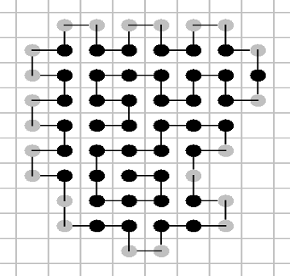
\includegraphics[width=1.5in]{figures/ibeabestresults.png}
	\caption{best solution found bu the IBEA with 40 topological neighbors.}
	\label{bestSolutionIBEA}
\end{figure}


\begin{figure}[ht]
	\centering
	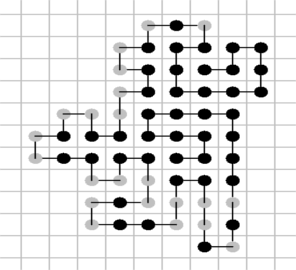
\includegraphics[width=1.5in]{figures/nsgaiibestresults.png}
	\caption{best solution found bu the NSGAII with 32 topological neighbors.}
	\label{bestSolutionNSGAII}
\end{figure}


\section{Related Works} \label{sec:related_works}


This section presents three works that have strategy implementations for multi-objective algorithms applied to the PSP problem, and served as base to propose this work.


Li et al. \cite{li2012genetic} developed a mono-objective EA combined to a strategy of local search based on pull moves to the 2D-HP model \cite{lesh2003complete}. The author made experiments using chains of 20 to 64 residues. They compare the obtained results with the results of others studies and conclude that the proposed approach appear to be efficient when compared with other strategies used in previous studies.


The study developed by Gabriel et al \cite{gabriel2012algoritmos} proposes a multi-objective EA for the PSP problem using the HP model, which evaluates the number of topological neighbors, as the compression degree of a conformation. The studies of the authors concluded that their study could find solutions with the same number of topological neighbors as a mono-objective algorithm using small populations than related in other approaches, and demonstrate a positive effect in the use of a multi-objective approach.


Soares et al \cite{soares2011investigating} proposed a multi-objective GA using the Van der Walls and Electrostatic Energy formulas as methods for the energy calculation. The authors made experiments with the proposed algorithm and also with the NSGAII \cite{deb2002fast} and concluded that the proposed algorithm presented better results when compared to the NSGAII.


\section{Conclusion and Future Works} \label{sec:conclusion}


From the experiments made, it was possible to conclude the application of a multi-objective approach for the PSP problem presented difference between the two evaluated algorithms IBEA and NSGAII. It was possible to verify a difference in the hypervolume values between the algorithms. However, this difference became clear only when comparing the energy objective. When comparing the IBEA algorithm with other studies with the same sequence of amino-acids, what was observed is that for 7 studies, 5 obtained worst results than IBEA and only 2 obtained a better result. Finally, it was also concluded the crossover operator that showed better results was the TwoPoints providing the best results for both algorithms when used.


Future works includes the exploration of more techniques of selection, crossover and mutation. The use use of Hyper-Heuristics for the selection of operators. Realize tests with other sequences of amino-acids. Make use of other search techniques. The addition of a graphic interface that make possible the interaction of a specialized user of the problem domain with the MOEAs.


\bibliographystyle{IEEEtran}
\bibliography{references}

% that's all folks
\end{document}